\documentclass[12pt, a4paper]{article}
\usepackage{amsmath}
\usepackage{amssymb, amsfonts}
\usepackage[utf8]{inputenc}    % Soporte para caracteres especiales
\usepackage{amsfonts}
%\usepackage[right=3cm, left=2.5cm, top=3cm, bottom=3.5cm]{geometry}
\usepackage{geometry}
\geometry{margin=2.5cm}
\usepackage{graphicx}
\usepackage{float}
%\usepackage{hyperref}          % Enlaces y referencias
%\usepackage[style=apa]{biblatex}
%\usepackage{csquotes}          % Manejo de citas (opcional, útil para biblatex)
%\addbibresource{references.bib}
%\usepackage[spanish]{babel}

\usepackage[style=apa, backend=biber]{biblatex}
\DeclareLanguageMapping{spanish}{spanish-apa}
\addbibresource{references.bib}
\usepackage[T1]{fontenc}
\usepackage{csquotes}
\usepackage{setspace}


\usepackage{tikz}
\usetikzlibrary{arrows.meta, decorations.markings, positioning}


\title{Título del documento}
\author{Autor del documento}

\begin{document}

\begin{titlepage}
\begin{center}

% --- Logos y encabezado superior ---
\begin{minipage}{0.2\textwidth}
    \begin{flushleft}
        \includegraphics[width=\linewidth]{img/logounp.png}
    \end{flushleft}
\end{minipage}
\begin{minipage}{0.6\textwidth}
    \begin{center}
        \vspace{2cm}
        \textbf{\large UNIVERSIDAD NACIONAL DE PIURA}\\[0.3cm]
        \vspace{0.3cm}
        \textbf{\large FACULTAD DE CIENCIAS}\\[0.3cm]
        \vspace{1cm}
        \textbf{ ESCUELA PROFESIONAL DE FÍSICA}
    \end{center}
\end{minipage}
\begin{minipage}{0.17\textwidth}
    \begin{flushright}
        \includegraphics[width=\linewidth]{img/physics.png}
    \end{flushright}
\end{minipage}

\vspace{2cm}

% --- Título ---
{\Large \textbf{
    Laboratorio virtual de espectrofotometría UV-VIS    
}}\\[1.5cm]

% --- Docente ---
\textbf{Docente:}\\ Dr. Quispe Moreno, Gustavo\\[1cm]

% --- Alumnos ---
\textbf{Alumnos:}\\
Torres Tarrillo, Rober E.\\
Carcamo Calderon, Andri, J.\\

% --- Fecha y lugar ---
\vfill
Piura, Diciembre 2025

\end{center}
\end{titlepage}
\begin{abstract}
La presente monografía aborda de manera teórica los fundamentos cuánticos de la \textbf{espectroscopía de microondas}, técnica espectroscópica que permite el estudio de los \textbf{niveles rotacionales de moléculas polares}. A partir de la ecuación de Schrödinger para el \textit{rotor rígido lineal}, se deducen las \textbf{energías de los niveles rotacionales} y se analiza la aparición de las líneas espectrales mediante las reglas de selección permitidas por el momento dipolar. 

Se desarrolla la expresión general para la \textbf{constante rotacional} $B = \frac{h}{8\pi^2 I c}$, relacionándola con el \textbf{momento de inercia molecular} y las \textbf{longitudes de enlace}, mostrando cómo la espectroscopía de microondas constituye una herramienta precisa para determinar parámetros estructurales a nivel cuántico. Además, se extiende el modelo al \textbf{rotor no rígido}, incorporando correcciones centrífugas que explican la separación no uniforme de las líneas espectrales observadas experimentalmente.

El trabajo incluye la deducción de las \textbf{reglas de selección rotacionales} $(\Delta J = \pm 1)$, el análisis del espectro rotacional de moléculas diatómicas como HCl y CO, así como la discusión de las diferencias entre \textbf{rotores lineales, simétricos y asimétricos}. Finalmente, se presentan aplicaciones relevantes en la \textbf{astrofísica molecular}, la \textbf{identificación espectral de compuestos gaseosos} y la \textbf{determinación de constantes moleculares fundamentales}. 

El enfoque es enteramente teórico, sin componente experimental, y se acompaña de las deducciones matemáticas necesarias para comprender la naturaleza cuántica de las transiciones rotacionales en el dominio de las microondas.
\end{abstract}
\newpage
\tableofcontents
\newpage
\section{Introducción}

La detección sensible y específica de ácido desoxirribonucleico (ADN) constituye un aspecto fundamental en diversas áreas de la ciencia y la tecnología, como la biomedicina, el diagnóstico molecular, la genética y el desarrollo de biosensores. La identificación de secuencias de ADN a bajas concentraciones es esencial para la detección temprana de enfermedades, el análisis genético y el monitoreo de procesos biológicos. No obstante, muchos de los métodos convencionales utilizados para este fin, como la reacción en cadena de la polimerasa (PCR) o las técnicas basadas en fluorescencia, requieren procedimientos complejos, el uso de marcadores químicos y un control experimental riguroso, lo que incrementa el costo y el tiempo de análisis.

La espectroscopía Raman se presenta como una técnica analítica capaz de proporcionar información molecular detallada a partir de las vibraciones características de las moléculas. Sin embargo, su aplicación directa está limitada por la baja intensidad de la señal Raman. Para superar esta limitación, se ha desarrollado la espectroscopía Raman mejorada en superficie (Surface-Enhanced Raman Spectroscopy, SERS), la cual permite un incremento significativo de la señal Raman mediante la interacción de las moléculas con superficies metálicas nanostructuradas, especialmente aquellas basadas en metales nobles como la plata.

En los últimos años, los métodos de detección sin marcadores (label-free) han cobrado especial relevancia debido a que permiten identificar biomoléculas sin la necesidad de etiquetas externas, reduciendo la complejidad experimental y posibles interferencias. En este contexto, el crecimiento de nanopartículas de plata mediado por ADN constituye una estrategia eficiente para la generación de regiones de alto campo electromagnético, conocidas como \textit{hot spots}, que potencian la sensibilidad de la técnica SERS y posibilitan la detección de ADN a muy bajas concentraciones.

En función de lo expuesto, la presente monografía se plantea los siguientes objetivos:

\subsection*{Objetivo general}
\begin{enumerate}
    \item Analizar el principio y la eficacia de la espectroscopía Raman mejorada en superficie sin marcadores para la detección sensible de ADN mediante el crecimiento de nanopartículas de plata mediado por ADN.
\end{enumerate}

\subsection*{Objetivos específicos}
\begin{enumerate}
    \item Explicar el fundamento físico de la espectroscopía Raman y de la espectroscopía Raman mejorada en superficie (SERS).
    \item Describir el papel del ADN en el crecimiento de nanopartículas de plata.
    \item Analizar el mecanismo de detección sin marcadores (\textit{label-free}) aplicado a la detección de ADN.
    \item Identificar las principales ventajas y limitaciones del método propuesto.
\end{enumerate}

\section{Aplicaciones y equipos}
\subsection{Equipos y principio de funcionamiento}

La espectroscopía de microondas utiliza una variedad de equipos diseñados para generar, detectar y analizar la radiación electromagnética en el rango de 1 a 300~GHz. A continuación se describen los principales dispositivos empleados en investigación y sus principios de operación.

\subsubsection{Espectrómetro de microondas de cavidad resonante}
Este tipo de espectrómetro utiliza una cavidad metálica cerrada en la cual se establece una onda estacionaria de microondas.  
Cuando una muestra gaseosa con moléculas polares se introduce en la cavidad, la absorción de radiación ocurre únicamente a frecuencias resonantes con las transiciones rotacionales.

\vspace{12pt}
\textbf{Principio de funcionamiento:}
\begin{itemize}
    \item Un generador de microondas (magnetrón o klystron) produce radiación coherente.
    \item La radiación es dirigida hacia la cavidad resonante donde se encuentra la muestra.
    \item Un detector de microondas mide la intensidad transmitida o reflejada.
    \item Las pérdidas de energía en resonancia corresponden a transiciones rotacionales.
\end{itemize}

Este tipo de espectrómetro fue ampliamente utilizado en los primeros estudios de HCl, CO y NH$_3$, permitiendo determinar con precisión sus constantes rotacionales.

\begin{figure}[H]
\centering
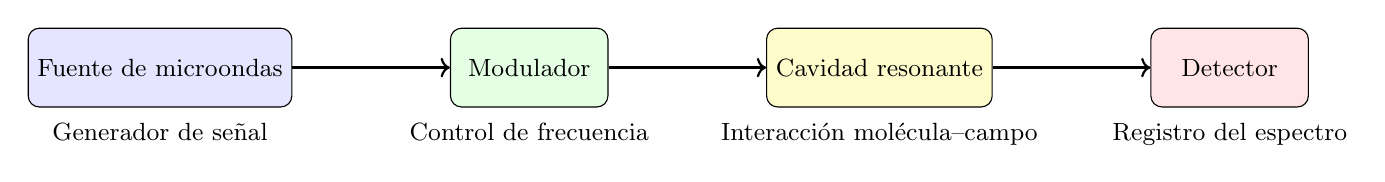
\begin{tikzpicture}[scale=1.1, every node/.style={font=\small}]
% Fuente de microondas
\node (fuente) at (0,0) [draw, rectangle, rounded corners, minimum width=2cm, minimum height=1cm, fill=blue!10] {Fuente de microondas};
\node[below=2pt of fuente] {Generador de señal};

% Modulador
\node (modulador) [right=2cm of fuente, draw, rectangle, rounded corners, minimum width=2cm, minimum height=1cm, fill=green!10] {Modulador};
\node[below=2pt of modulador] {Control de frecuencia};

% Cavidad resonante
\node (cavidad) [right=2cm of modulador, draw, rectangle, rounded corners, minimum width=2cm, minimum height=1cm, fill=yellow!20] {Cavidad resonante};
\node[below=2pt of cavidad] {Interacción molécula–campo};

% Detector
\node (detector) [right=2cm of cavidad, draw, rectangle, rounded corners, minimum width=2cm, minimum height=1cm, fill=red!10] {Detector};
\node[below=2pt of detector] {Registro del espectro};

% Flechas de conexión
\draw[->, thick] (fuente) -- (modulador);
\draw[->, thick] (modulador) -- (cavidad);
\draw[->, thick] (cavidad) -- (detector);
\end{tikzpicture}
\caption{Esquema general de un espectrómetro de microondas.}
\label{fig:espectrometro}
\end{figure}

\begin{figure}[H]
    \centering
    \includegraphics[width=0.8\textwidth]{img/microwave.png}    
    \caption{Espectrómetro de microondas con cavidad resonante. (\cite{quimicamoderna_microondas})}
\end{figure}


\subsubsection{Espectrómetro de Transformada de Fourier de microondas (FTMW)}
El espectrómetro FTMW (\textit{Fourier Transform Microwave Spectrometer}) utiliza pulsos breves de microondas que excitan las moléculas, y posteriormente mide la señal de emisión libre (\textit{free induction decay}) en el dominio del tiempo.  
Mediante una transformada de Fourier se obtiene el espectro en el dominio de la frecuencia.

\textbf{Principio de funcionamiento:}
\begin{itemize}
    \item Un pulso de microondas coherente excita las transiciones rotacionales.
    \item Las moléculas reemiten radiación coherente cuando regresan a su estado base.
    \item Una antena o guía de onda detecta esta señal de emisión libre.
    \item La transformada de Fourier convierte la señal temporal en el espectro de frecuencia.
\end{itemize}

Este método proporciona una resolución extremadamente alta (del orden de kHz) y permite estudiar mezclas complejas o especies reactivas generadas en celdas de descarga.

\begin{figure}[h]
    \centering
    \includegraphics[width=0.8\textwidth]{img/ftmw.png}
    \caption{Espectro de un FTMW. (\cite{kiel_ftmw_spectrometer})}
\end{figure}

\subsubsection{Radiotelescopios para observaciones astronómicas}
En astronomía, los radiotelescopios detectan la radiación de microondas emitida por moléculas en el espacio interestelar. Las antenas parabólicas concentran la radiación hacia receptores sensibles refrigerados criogénicamente.

\textbf{Principio de funcionamiento:}
\begin{itemize}
    \item La antena parabólica concentra las ondas de microondas hacia el receptor.
    \item El receptor (normalmente un \textit{mezclador heterodino}) convierte la señal a una frecuencia intermedia.
    \item Un analizador espectral o sistema digital extrae las líneas de emisión rotacionales.
    \item Los datos se procesan para determinar la intensidad, desplazamiento Doppler y abundancia molecular.
\end{itemize}

Ejemplos notables de equipos son el \textbf{Atacama Large Millimeter/submillimeter Array (ALMA)} en Chile y el \textbf{Green Bank Telescope (GBT)} en Estados Unidos.

\begin{figure}[H]
    \centering
    \includegraphics[width=0.8\textwidth]{img/alma.png}
    \caption{ALMA. (\cite{cooper_alma_space})}
\end{figure}

\begin{figure}[H]
    \centering
    \includegraphics[width=0.8\textwidth]{img/gbt.png}
    \caption{GBT. (\cite{nrao_gbt})}
\end{figure}



\subsubsection{Analizadores vectoriales de redes (VNA)}
Los analizadores de redes se utilizan para estudiar materiales o sistemas mediante la medición de parámetros de dispersión (\(S_{11}, S_{21}\)) de microondas incidentes.  
En el contexto espectroscópico, permiten estudiar la respuesta dieléctrica y la absorción en gases o sólidos.

\textbf{Principio de funcionamiento:}
\begin{itemize}
    \item El VNA genera una señal de microondas de frecuencia variable.
    \item Mide las señales reflejadas y transmitidas a través de la muestra.
    \item Calcula los parámetros \(S_{ij}\), que contienen información sobre la absorción y la fase.
    \item De estos parámetros se puede inferir la constante dieléctrica y las resonancias rotacionales.
\end{itemize}

Estos instrumentos son ampliamente empleados en ingeniería y en el desarrollo de sensores de microondas aplicados a biomedicina y materiales.

\begin{figure}[H]
    \centering
    \includegraphics[width=0.8\textwidth]{img/vna.png}
    \caption{VNA. (\cite{rohdeschwarz_lcr_vna})}
\end{figure}

\subsubsection{Sistemas láser acoplados a espectroscopía rotacional}
En investigaciones avanzadas, los espectrómetros de microondas pueden acoplarse a láseres de alta precisión para excitar o detectar estados rotacionales y vibracionales simultáneamente.  
Este enfoque es fundamental para estudiar moléculas con estructuras electrónicas complejas.

\begin{figure}[H]
    \centering
    \includegraphics[width=0.8\textwidth]{img/brown.png}
    \caption{Esquema de un espectrómetro de microondas de transformada de Fourier con pulso chirpado, introducido por Brown \textit{et al.} (2008). 
    Un pulso de microondas de 12\,GHz de ancho de banda (de 1\,$\mu$s de duración) es generado por un generador de formas de onda arbitrarias (AWG), convertido a frecuencias en el rango de 6.8--18.5\,GHz y amplificado hasta varios cientos de vatios (1), antes de ingresar a la cámara del haz molecular (2). 
    La decadencia de inducción libre coherente (FID) de las moléculas excitadas, que contiene la información espectral, es posteriormente registrada y analizada mediante un osciloscopio digital de alta velocidad. 
    Reproducido con permiso de \cite{brown2008}.}
    \label{fig:chirped_spectrometer}
\end{figure}


\textbf{Ejemplo:}
\begin{itemize}
    \item Sistemas \textit{Chirped Pulse FTMW}, que usan pulsos amplios en frecuencia (1–20~GHz) para cubrir grandes regiones espectrales.
    \begin{figure}
        \centering
        \includegraphics[width=0.5\textwidth]{img/cpftmw.png}
        \caption{Chiperd Pulse FTMW}
    \end{figure}
    \item Equipos \textit{Lamb-dip microwave} que permiten mediciones hiperfinas de alta resolución.
\end{itemize}

\vspace{1em}
En conjunto, estos equipos permiten cubrir desde la caracterización básica de moléculas simples hasta el estudio de sistemas astrofísicos y materiales avanzados, consolidando a la espectroscopía de microondas como una herramienta esencial en la física moderna.

\subsection{Aplicaciones en distintas ramas y equipos}

La espectroscopía de microondas posee un amplio rango de aplicaciones en la investigación científica y tecnológica. Gracias a su alta resolución, permite obtener información precisa sobre las propiedades estructurales y dinámicas de las moléculas, así como sobre su interacción con campos electromagnéticos.

\subsubsection{Aplicaciones en química}
En química molecular, la espectroscopía rotacional es una herramienta esencial para determinar parámetros estructurales como la longitud de enlace, el momento dipolar y el ángulo de enlace.  
Ejemplos destacados incluyen:
\begin{itemize}
    \item Determinación de la longitud del enlace H–Cl en el ácido clorhídrico (HCl) a partir de su constante rotacional \( B \).
    \item Estudio de moléculas como H$_2$O y NH$_3$ para obtener su geometría angular.
    \item Análisis de moléculas orgánicas volátiles como el etanol (C$_2$H$_5$OH) o el formaldehído (H$_2$CO).
\end{itemize}
\textbf{Equipos utilizados:}
\begin{itemize}
    \item Espectrómetro de microondas de cavidad resonante.
    \item Espectrómetro de transformada de Fourier (FTMW).
    \item Celdas de descarga y sistemas criogénicos para generar especies reactivas.
\end{itemize}

\subsubsection{Aplicaciones en física}
En física cuántica y molecular, la espectroscopía de microondas permite comprobar modelos teóricos del rotor rígido y no rígido, estudiar acoplamientos espín-rotación y analizar efectos isotópicos.  
Ejemplos representativos:
\begin{itemize}
    \item Verificación de los niveles rotacionales en CO y N$_2$O.
    \item Determinación experimental del momento de inercia y comparación con resultados teóricos.
    \item Observación del desdoblamiento hiperfino en el radical OH.
\end{itemize}
\textbf{Equipos utilizados:}
\begin{itemize}
    \item Espectrómetros de cavidad resonante de alta precisión.
    \item Espectrómetros FTMW acoplados a fuentes láser.
\end{itemize}

\subsubsection{Aplicaciones en astronomía}
En astronomía, las transiciones rotacionales en el rango de microondas permiten identificar moléculas en el medio interestelar y estudiar la composición de atmósferas planetarias.  
Ejemplos:
\begin{itemize}
    \item Detección de CO, HCN y H$_2$O en nubes moleculares interestelares.
    \item Identificación de moléculas orgánicas complejas en regiones de formación estelar como Orión KL.
    \item Análisis de isótopos en moléculas como $^{13}$CO y C$^{18}$O.
\end{itemize}
\textbf{Equipos utilizados:}
\begin{itemize}
    \item Radiotelescopios como el \textbf{ALMA} y el \textbf{Green Bank Telescope (GBT)}.
    \item Espectrómetros acoplados a antenas parabólicas de alta sensibilidad.
\end{itemize}

\subsubsection{Aplicaciones en ingeniería y tecnología}
Los principios de la espectroscopía de microondas también se aplican en el desarrollo de sistemas tecnológicos de comunicación, sensores y diagnóstico.  
Ejemplos:
\begin{itemize}
    \item Diseño de sensores de humedad y densidad basados en absorción de microondas.
    \item Control de calidad industrial mediante medición dieléctrica.
    \item Aplicación de principios de dispersión de microondas en radares Doppler y sistemas médicos de diagnóstico.
\end{itemize}
\textbf{Equipos utilizados:}
\begin{itemize}
    \item Analizadores vectoriales de redes (VNA).
    \item Sensores dieléctricos y espectrómetros portátiles.
    \item Sistemas de radar de banda ancha y cámaras de microondas.
\end{itemize}

\subsubsection{Síntesis de aplicaciones}
La Tabla~\ref{tab:aplicaciones} resume las principales áreas de aplicación junto con ejemplos y equipos característicos.

\begin{table}[H]
\centering
\caption{Resumen de aplicaciones de la espectroscopía de microondas}
\label{tab:aplicaciones}
\begin{tabular}{|p{3cm}|p{5cm}|p{5cm}|}
\hline
\textbf{Área} & \textbf{Ejemplos de aplicación} & \textbf{Equipos utilizados} \\
\hline
Química & Geometría molecular de HCl, H$_2$O, NH$_3$ & FTMW, cavidad resonante \\
\hline
Física & Niveles rotacionales de CO, N$_2$O; acoplamiento espín-rotación & Cavidad resonante, espectroscopía láser \\
\hline
Astronomía & Detección de CO, HCN, H$_2$O en nubes moleculares & Radiotelescopios (ALMA, GBT) \\
\hline
Ingeniería & Sensores dieléctricos, radares, diagnóstico médico & Analizador de redes (VNA), sensores de microondas \\
\hline
\end{tabular}
\end{table}

En conjunto, estas aplicaciones evidencian la naturaleza interdisciplinaria de la espectroscopía de microondas y su papel clave en el avance de la física molecular, la química estructural, la radioastronomía y la ingeniería moderna.


% \section{Aplicaciones y equipos}
\subsection{Equipos y principio de funcionamiento}

La espectroscopía de microondas utiliza una variedad de equipos diseñados para generar, detectar y analizar la radiación electromagnética en el rango de 1 a 300~GHz. A continuación se describen los principales dispositivos empleados en investigación y sus principios de operación.

\subsubsection{Espectrómetro de microondas de cavidad resonante}
Este tipo de espectrómetro utiliza una cavidad metálica cerrada en la cual se establece una onda estacionaria de microondas.  
Cuando una muestra gaseosa con moléculas polares se introduce en la cavidad, la absorción de radiación ocurre únicamente a frecuencias resonantes con las transiciones rotacionales.

\vspace{12pt}
\textbf{Principio de funcionamiento:}
\begin{itemize}
    \item Un generador de microondas (magnetrón o klystron) produce radiación coherente.
    \item La radiación es dirigida hacia la cavidad resonante donde se encuentra la muestra.
    \item Un detector de microondas mide la intensidad transmitida o reflejada.
    \item Las pérdidas de energía en resonancia corresponden a transiciones rotacionales.
\end{itemize}

Este tipo de espectrómetro fue ampliamente utilizado en los primeros estudios de HCl, CO y NH$_3$, permitiendo determinar con precisión sus constantes rotacionales.

\begin{figure}[H]
\centering
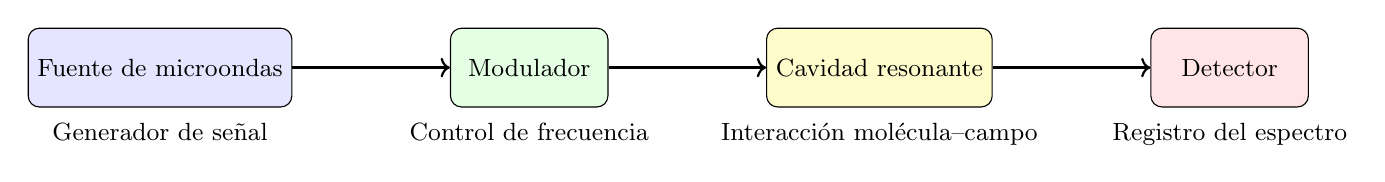
\begin{tikzpicture}[scale=1.1, every node/.style={font=\small}]
% Fuente de microondas
\node (fuente) at (0,0) [draw, rectangle, rounded corners, minimum width=2cm, minimum height=1cm, fill=blue!10] {Fuente de microondas};
\node[below=2pt of fuente] {Generador de señal};

% Modulador
\node (modulador) [right=2cm of fuente, draw, rectangle, rounded corners, minimum width=2cm, minimum height=1cm, fill=green!10] {Modulador};
\node[below=2pt of modulador] {Control de frecuencia};

% Cavidad resonante
\node (cavidad) [right=2cm of modulador, draw, rectangle, rounded corners, minimum width=2cm, minimum height=1cm, fill=yellow!20] {Cavidad resonante};
\node[below=2pt of cavidad] {Interacción molécula–campo};

% Detector
\node (detector) [right=2cm of cavidad, draw, rectangle, rounded corners, minimum width=2cm, minimum height=1cm, fill=red!10] {Detector};
\node[below=2pt of detector] {Registro del espectro};

% Flechas de conexión
\draw[->, thick] (fuente) -- (modulador);
\draw[->, thick] (modulador) -- (cavidad);
\draw[->, thick] (cavidad) -- (detector);
\end{tikzpicture}
\caption{Esquema general de un espectrómetro de microondas.}
\label{fig:espectrometro}
\end{figure}

\begin{figure}[H]
    \centering
    \includegraphics[width=0.8\textwidth]{img/microwave.png}    
    \caption{Espectrómetro de microondas con cavidad resonante. (\cite{quimicamoderna_microondas})}
\end{figure}


\subsubsection{Espectrómetro de Transformada de Fourier de microondas (FTMW)}
El espectrómetro FTMW (\textit{Fourier Transform Microwave Spectrometer}) utiliza pulsos breves de microondas que excitan las moléculas, y posteriormente mide la señal de emisión libre (\textit{free induction decay}) en el dominio del tiempo.  
Mediante una transformada de Fourier se obtiene el espectro en el dominio de la frecuencia.

\textbf{Principio de funcionamiento:}
\begin{itemize}
    \item Un pulso de microondas coherente excita las transiciones rotacionales.
    \item Las moléculas reemiten radiación coherente cuando regresan a su estado base.
    \item Una antena o guía de onda detecta esta señal de emisión libre.
    \item La transformada de Fourier convierte la señal temporal en el espectro de frecuencia.
\end{itemize}

Este método proporciona una resolución extremadamente alta (del orden de kHz) y permite estudiar mezclas complejas o especies reactivas generadas en celdas de descarga.

\begin{figure}[h]
    \centering
    \includegraphics[width=0.8\textwidth]{img/ftmw.png}
    \caption{Espectro de un FTMW. (\cite{kiel_ftmw_spectrometer})}
\end{figure}

\subsubsection{Radiotelescopios para observaciones astronómicas}
En astronomía, los radiotelescopios detectan la radiación de microondas emitida por moléculas en el espacio interestelar. Las antenas parabólicas concentran la radiación hacia receptores sensibles refrigerados criogénicamente.

\textbf{Principio de funcionamiento:}
\begin{itemize}
    \item La antena parabólica concentra las ondas de microondas hacia el receptor.
    \item El receptor (normalmente un \textit{mezclador heterodino}) convierte la señal a una frecuencia intermedia.
    \item Un analizador espectral o sistema digital extrae las líneas de emisión rotacionales.
    \item Los datos se procesan para determinar la intensidad, desplazamiento Doppler y abundancia molecular.
\end{itemize}

Ejemplos notables de equipos son el \textbf{Atacama Large Millimeter/submillimeter Array (ALMA)} en Chile y el \textbf{Green Bank Telescope (GBT)} en Estados Unidos.

\begin{figure}[H]
    \centering
    \includegraphics[width=0.8\textwidth]{img/alma.png}
    \caption{ALMA. (\cite{cooper_alma_space})}
\end{figure}

\begin{figure}[H]
    \centering
    \includegraphics[width=0.8\textwidth]{img/gbt.png}
    \caption{GBT. (\cite{nrao_gbt})}
\end{figure}



\subsubsection{Analizadores vectoriales de redes (VNA)}
Los analizadores de redes se utilizan para estudiar materiales o sistemas mediante la medición de parámetros de dispersión (\(S_{11}, S_{21}\)) de microondas incidentes.  
En el contexto espectroscópico, permiten estudiar la respuesta dieléctrica y la absorción en gases o sólidos.

\textbf{Principio de funcionamiento:}
\begin{itemize}
    \item El VNA genera una señal de microondas de frecuencia variable.
    \item Mide las señales reflejadas y transmitidas a través de la muestra.
    \item Calcula los parámetros \(S_{ij}\), que contienen información sobre la absorción y la fase.
    \item De estos parámetros se puede inferir la constante dieléctrica y las resonancias rotacionales.
\end{itemize}

Estos instrumentos son ampliamente empleados en ingeniería y en el desarrollo de sensores de microondas aplicados a biomedicina y materiales.

\begin{figure}[H]
    \centering
    \includegraphics[width=0.8\textwidth]{img/vna.png}
    \caption{VNA. (\cite{rohdeschwarz_lcr_vna})}
\end{figure}

\subsubsection{Sistemas láser acoplados a espectroscopía rotacional}
En investigaciones avanzadas, los espectrómetros de microondas pueden acoplarse a láseres de alta precisión para excitar o detectar estados rotacionales y vibracionales simultáneamente.  
Este enfoque es fundamental para estudiar moléculas con estructuras electrónicas complejas.

\begin{figure}[H]
    \centering
    \includegraphics[width=0.8\textwidth]{img/brown.png}
    \caption{Esquema de un espectrómetro de microondas de transformada de Fourier con pulso chirpado, introducido por Brown \textit{et al.} (2008). 
    Un pulso de microondas de 12\,GHz de ancho de banda (de 1\,$\mu$s de duración) es generado por un generador de formas de onda arbitrarias (AWG), convertido a frecuencias en el rango de 6.8--18.5\,GHz y amplificado hasta varios cientos de vatios (1), antes de ingresar a la cámara del haz molecular (2). 
    La decadencia de inducción libre coherente (FID) de las moléculas excitadas, que contiene la información espectral, es posteriormente registrada y analizada mediante un osciloscopio digital de alta velocidad. 
    Reproducido con permiso de \cite{brown2008}.}
    \label{fig:chirped_spectrometer}
\end{figure}


\textbf{Ejemplo:}
\begin{itemize}
    \item Sistemas \textit{Chirped Pulse FTMW}, que usan pulsos amplios en frecuencia (1–20~GHz) para cubrir grandes regiones espectrales.
    \begin{figure}
        \centering
        \includegraphics[width=0.5\textwidth]{img/cpftmw.png}
        \caption{Chiperd Pulse FTMW}
    \end{figure}
    \item Equipos \textit{Lamb-dip microwave} que permiten mediciones hiperfinas de alta resolución.
\end{itemize}

\vspace{1em}
En conjunto, estos equipos permiten cubrir desde la caracterización básica de moléculas simples hasta el estudio de sistemas astrofísicos y materiales avanzados, consolidando a la espectroscopía de microondas como una herramienta esencial en la física moderna.

\subsection{Aplicaciones en distintas ramas y equipos}

La espectroscopía de microondas posee un amplio rango de aplicaciones en la investigación científica y tecnológica. Gracias a su alta resolución, permite obtener información precisa sobre las propiedades estructurales y dinámicas de las moléculas, así como sobre su interacción con campos electromagnéticos.

\subsubsection{Aplicaciones en química}
En química molecular, la espectroscopía rotacional es una herramienta esencial para determinar parámetros estructurales como la longitud de enlace, el momento dipolar y el ángulo de enlace.  
Ejemplos destacados incluyen:
\begin{itemize}
    \item Determinación de la longitud del enlace H–Cl en el ácido clorhídrico (HCl) a partir de su constante rotacional \( B \).
    \item Estudio de moléculas como H$_2$O y NH$_3$ para obtener su geometría angular.
    \item Análisis de moléculas orgánicas volátiles como el etanol (C$_2$H$_5$OH) o el formaldehído (H$_2$CO).
\end{itemize}
\textbf{Equipos utilizados:}
\begin{itemize}
    \item Espectrómetro de microondas de cavidad resonante.
    \item Espectrómetro de transformada de Fourier (FTMW).
    \item Celdas de descarga y sistemas criogénicos para generar especies reactivas.
\end{itemize}

\subsubsection{Aplicaciones en física}
En física cuántica y molecular, la espectroscopía de microondas permite comprobar modelos teóricos del rotor rígido y no rígido, estudiar acoplamientos espín-rotación y analizar efectos isotópicos.  
Ejemplos representativos:
\begin{itemize}
    \item Verificación de los niveles rotacionales en CO y N$_2$O.
    \item Determinación experimental del momento de inercia y comparación con resultados teóricos.
    \item Observación del desdoblamiento hiperfino en el radical OH.
\end{itemize}
\textbf{Equipos utilizados:}
\begin{itemize}
    \item Espectrómetros de cavidad resonante de alta precisión.
    \item Espectrómetros FTMW acoplados a fuentes láser.
\end{itemize}

\subsubsection{Aplicaciones en astronomía}
En astronomía, las transiciones rotacionales en el rango de microondas permiten identificar moléculas en el medio interestelar y estudiar la composición de atmósferas planetarias.  
Ejemplos:
\begin{itemize}
    \item Detección de CO, HCN y H$_2$O en nubes moleculares interestelares.
    \item Identificación de moléculas orgánicas complejas en regiones de formación estelar como Orión KL.
    \item Análisis de isótopos en moléculas como $^{13}$CO y C$^{18}$O.
\end{itemize}
\textbf{Equipos utilizados:}
\begin{itemize}
    \item Radiotelescopios como el \textbf{ALMA} y el \textbf{Green Bank Telescope (GBT)}.
    \item Espectrómetros acoplados a antenas parabólicas de alta sensibilidad.
\end{itemize}

\subsubsection{Aplicaciones en ingeniería y tecnología}
Los principios de la espectroscopía de microondas también se aplican en el desarrollo de sistemas tecnológicos de comunicación, sensores y diagnóstico.  
Ejemplos:
\begin{itemize}
    \item Diseño de sensores de humedad y densidad basados en absorción de microondas.
    \item Control de calidad industrial mediante medición dieléctrica.
    \item Aplicación de principios de dispersión de microondas en radares Doppler y sistemas médicos de diagnóstico.
\end{itemize}
\textbf{Equipos utilizados:}
\begin{itemize}
    \item Analizadores vectoriales de redes (VNA).
    \item Sensores dieléctricos y espectrómetros portátiles.
    \item Sistemas de radar de banda ancha y cámaras de microondas.
\end{itemize}

\subsubsection{Síntesis de aplicaciones}
La Tabla~\ref{tab:aplicaciones} resume las principales áreas de aplicación junto con ejemplos y equipos característicos.

\begin{table}[H]
\centering
\caption{Resumen de aplicaciones de la espectroscopía de microondas}
\label{tab:aplicaciones}
\begin{tabular}{|p{3cm}|p{5cm}|p{5cm}|}
\hline
\textbf{Área} & \textbf{Ejemplos de aplicación} & \textbf{Equipos utilizados} \\
\hline
Química & Geometría molecular de HCl, H$_2$O, NH$_3$ & FTMW, cavidad resonante \\
\hline
Física & Niveles rotacionales de CO, N$_2$O; acoplamiento espín-rotación & Cavidad resonante, espectroscopía láser \\
\hline
Astronomía & Detección de CO, HCN, H$_2$O en nubes moleculares & Radiotelescopios (ALMA, GBT) \\
\hline
Ingeniería & Sensores dieléctricos, radares, diagnóstico médico & Analizador de redes (VNA), sensores de microondas \\
\hline
\end{tabular}
\end{table}

En conjunto, estas aplicaciones evidencian la naturaleza interdisciplinaria de la espectroscopía de microondas y su papel clave en el avance de la física molecular, la química estructural, la radioastronomía y la ingeniería moderna.


\section{Aplicaciones y equipos}
\subsection{Equipos y principio de funcionamiento}

La espectroscopía de microondas utiliza una variedad de equipos diseñados para generar, detectar y analizar la radiación electromagnética en el rango de 1 a 300~GHz. A continuación se describen los principales dispositivos empleados en investigación y sus principios de operación.

\subsubsection{Espectrómetro de microondas de cavidad resonante}
Este tipo de espectrómetro utiliza una cavidad metálica cerrada en la cual se establece una onda estacionaria de microondas.  
Cuando una muestra gaseosa con moléculas polares se introduce en la cavidad, la absorción de radiación ocurre únicamente a frecuencias resonantes con las transiciones rotacionales.

\vspace{12pt}
\textbf{Principio de funcionamiento:}
\begin{itemize}
    \item Un generador de microondas (magnetrón o klystron) produce radiación coherente.
    \item La radiación es dirigida hacia la cavidad resonante donde se encuentra la muestra.
    \item Un detector de microondas mide la intensidad transmitida o reflejada.
    \item Las pérdidas de energía en resonancia corresponden a transiciones rotacionales.
\end{itemize}

Este tipo de espectrómetro fue ampliamente utilizado en los primeros estudios de HCl, CO y NH$_3$, permitiendo determinar con precisión sus constantes rotacionales.

\begin{figure}[H]
\centering
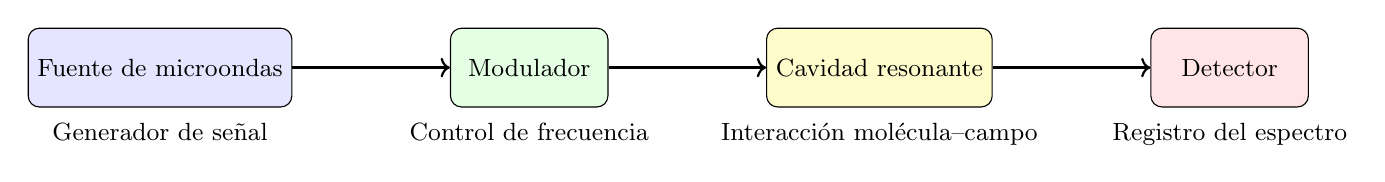
\begin{tikzpicture}[scale=1.1, every node/.style={font=\small}]
% Fuente de microondas
\node (fuente) at (0,0) [draw, rectangle, rounded corners, minimum width=2cm, minimum height=1cm, fill=blue!10] {Fuente de microondas};
\node[below=2pt of fuente] {Generador de señal};

% Modulador
\node (modulador) [right=2cm of fuente, draw, rectangle, rounded corners, minimum width=2cm, minimum height=1cm, fill=green!10] {Modulador};
\node[below=2pt of modulador] {Control de frecuencia};

% Cavidad resonante
\node (cavidad) [right=2cm of modulador, draw, rectangle, rounded corners, minimum width=2cm, minimum height=1cm, fill=yellow!20] {Cavidad resonante};
\node[below=2pt of cavidad] {Interacción molécula–campo};

% Detector
\node (detector) [right=2cm of cavidad, draw, rectangle, rounded corners, minimum width=2cm, minimum height=1cm, fill=red!10] {Detector};
\node[below=2pt of detector] {Registro del espectro};

% Flechas de conexión
\draw[->, thick] (fuente) -- (modulador);
\draw[->, thick] (modulador) -- (cavidad);
\draw[->, thick] (cavidad) -- (detector);
\end{tikzpicture}
\caption{Esquema general de un espectrómetro de microondas.}
\label{fig:espectrometro}
\end{figure}

\begin{figure}[H]
    \centering
    \includegraphics[width=0.8\textwidth]{img/microwave.png}    
    \caption{Espectrómetro de microondas con cavidad resonante. (\cite{quimicamoderna_microondas})}
\end{figure}


\subsubsection{Espectrómetro de Transformada de Fourier de microondas (FTMW)}
El espectrómetro FTMW (\textit{Fourier Transform Microwave Spectrometer}) utiliza pulsos breves de microondas que excitan las moléculas, y posteriormente mide la señal de emisión libre (\textit{free induction decay}) en el dominio del tiempo.  
Mediante una transformada de Fourier se obtiene el espectro en el dominio de la frecuencia.

\textbf{Principio de funcionamiento:}
\begin{itemize}
    \item Un pulso de microondas coherente excita las transiciones rotacionales.
    \item Las moléculas reemiten radiación coherente cuando regresan a su estado base.
    \item Una antena o guía de onda detecta esta señal de emisión libre.
    \item La transformada de Fourier convierte la señal temporal en el espectro de frecuencia.
\end{itemize}

Este método proporciona una resolución extremadamente alta (del orden de kHz) y permite estudiar mezclas complejas o especies reactivas generadas en celdas de descarga.

\begin{figure}[h]
    \centering
    \includegraphics[width=0.8\textwidth]{img/ftmw.png}
    \caption{Espectro de un FTMW. (\cite{kiel_ftmw_spectrometer})}
\end{figure}

\subsubsection{Radiotelescopios para observaciones astronómicas}
En astronomía, los radiotelescopios detectan la radiación de microondas emitida por moléculas en el espacio interestelar. Las antenas parabólicas concentran la radiación hacia receptores sensibles refrigerados criogénicamente.

\textbf{Principio de funcionamiento:}
\begin{itemize}
    \item La antena parabólica concentra las ondas de microondas hacia el receptor.
    \item El receptor (normalmente un \textit{mezclador heterodino}) convierte la señal a una frecuencia intermedia.
    \item Un analizador espectral o sistema digital extrae las líneas de emisión rotacionales.
    \item Los datos se procesan para determinar la intensidad, desplazamiento Doppler y abundancia molecular.
\end{itemize}

Ejemplos notables de equipos son el \textbf{Atacama Large Millimeter/submillimeter Array (ALMA)} en Chile y el \textbf{Green Bank Telescope (GBT)} en Estados Unidos.

\begin{figure}[H]
    \centering
    \includegraphics[width=0.8\textwidth]{img/alma.png}
    \caption{ALMA. (\cite{cooper_alma_space})}
\end{figure}

\begin{figure}[H]
    \centering
    \includegraphics[width=0.8\textwidth]{img/gbt.png}
    \caption{GBT. (\cite{nrao_gbt})}
\end{figure}



\subsubsection{Analizadores vectoriales de redes (VNA)}
Los analizadores de redes se utilizan para estudiar materiales o sistemas mediante la medición de parámetros de dispersión (\(S_{11}, S_{21}\)) de microondas incidentes.  
En el contexto espectroscópico, permiten estudiar la respuesta dieléctrica y la absorción en gases o sólidos.

\textbf{Principio de funcionamiento:}
\begin{itemize}
    \item El VNA genera una señal de microondas de frecuencia variable.
    \item Mide las señales reflejadas y transmitidas a través de la muestra.
    \item Calcula los parámetros \(S_{ij}\), que contienen información sobre la absorción y la fase.
    \item De estos parámetros se puede inferir la constante dieléctrica y las resonancias rotacionales.
\end{itemize}

Estos instrumentos son ampliamente empleados en ingeniería y en el desarrollo de sensores de microondas aplicados a biomedicina y materiales.

\begin{figure}[H]
    \centering
    \includegraphics[width=0.8\textwidth]{img/vna.png}
    \caption{VNA. (\cite{rohdeschwarz_lcr_vna})}
\end{figure}

\subsubsection{Sistemas láser acoplados a espectroscopía rotacional}
En investigaciones avanzadas, los espectrómetros de microondas pueden acoplarse a láseres de alta precisión para excitar o detectar estados rotacionales y vibracionales simultáneamente.  
Este enfoque es fundamental para estudiar moléculas con estructuras electrónicas complejas.

\begin{figure}[H]
    \centering
    \includegraphics[width=0.8\textwidth]{img/brown.png}
    \caption{Esquema de un espectrómetro de microondas de transformada de Fourier con pulso chirpado, introducido por Brown \textit{et al.} (2008). 
    Un pulso de microondas de 12\,GHz de ancho de banda (de 1\,$\mu$s de duración) es generado por un generador de formas de onda arbitrarias (AWG), convertido a frecuencias en el rango de 6.8--18.5\,GHz y amplificado hasta varios cientos de vatios (1), antes de ingresar a la cámara del haz molecular (2). 
    La decadencia de inducción libre coherente (FID) de las moléculas excitadas, que contiene la información espectral, es posteriormente registrada y analizada mediante un osciloscopio digital de alta velocidad. 
    Reproducido con permiso de \cite{brown2008}.}
    \label{fig:chirped_spectrometer}
\end{figure}


\textbf{Ejemplo:}
\begin{itemize}
    \item Sistemas \textit{Chirped Pulse FTMW}, que usan pulsos amplios en frecuencia (1–20~GHz) para cubrir grandes regiones espectrales.
    \begin{figure}
        \centering
        \includegraphics[width=0.5\textwidth]{img/cpftmw.png}
        \caption{Chiperd Pulse FTMW}
    \end{figure}
    \item Equipos \textit{Lamb-dip microwave} que permiten mediciones hiperfinas de alta resolución.
\end{itemize}

\vspace{1em}
En conjunto, estos equipos permiten cubrir desde la caracterización básica de moléculas simples hasta el estudio de sistemas astrofísicos y materiales avanzados, consolidando a la espectroscopía de microondas como una herramienta esencial en la física moderna.

\subsection{Aplicaciones en distintas ramas y equipos}

La espectroscopía de microondas posee un amplio rango de aplicaciones en la investigación científica y tecnológica. Gracias a su alta resolución, permite obtener información precisa sobre las propiedades estructurales y dinámicas de las moléculas, así como sobre su interacción con campos electromagnéticos.

\subsubsection{Aplicaciones en química}
En química molecular, la espectroscopía rotacional es una herramienta esencial para determinar parámetros estructurales como la longitud de enlace, el momento dipolar y el ángulo de enlace.  
Ejemplos destacados incluyen:
\begin{itemize}
    \item Determinación de la longitud del enlace H–Cl en el ácido clorhídrico (HCl) a partir de su constante rotacional \( B \).
    \item Estudio de moléculas como H$_2$O y NH$_3$ para obtener su geometría angular.
    \item Análisis de moléculas orgánicas volátiles como el etanol (C$_2$H$_5$OH) o el formaldehído (H$_2$CO).
\end{itemize}
\textbf{Equipos utilizados:}
\begin{itemize}
    \item Espectrómetro de microondas de cavidad resonante.
    \item Espectrómetro de transformada de Fourier (FTMW).
    \item Celdas de descarga y sistemas criogénicos para generar especies reactivas.
\end{itemize}

\subsubsection{Aplicaciones en física}
En física cuántica y molecular, la espectroscopía de microondas permite comprobar modelos teóricos del rotor rígido y no rígido, estudiar acoplamientos espín-rotación y analizar efectos isotópicos.  
Ejemplos representativos:
\begin{itemize}
    \item Verificación de los niveles rotacionales en CO y N$_2$O.
    \item Determinación experimental del momento de inercia y comparación con resultados teóricos.
    \item Observación del desdoblamiento hiperfino en el radical OH.
\end{itemize}
\textbf{Equipos utilizados:}
\begin{itemize}
    \item Espectrómetros de cavidad resonante de alta precisión.
    \item Espectrómetros FTMW acoplados a fuentes láser.
\end{itemize}

\subsubsection{Aplicaciones en astronomía}
En astronomía, las transiciones rotacionales en el rango de microondas permiten identificar moléculas en el medio interestelar y estudiar la composición de atmósferas planetarias.  
Ejemplos:
\begin{itemize}
    \item Detección de CO, HCN y H$_2$O en nubes moleculares interestelares.
    \item Identificación de moléculas orgánicas complejas en regiones de formación estelar como Orión KL.
    \item Análisis de isótopos en moléculas como $^{13}$CO y C$^{18}$O.
\end{itemize}
\textbf{Equipos utilizados:}
\begin{itemize}
    \item Radiotelescopios como el \textbf{ALMA} y el \textbf{Green Bank Telescope (GBT)}.
    \item Espectrómetros acoplados a antenas parabólicas de alta sensibilidad.
\end{itemize}

\subsubsection{Aplicaciones en ingeniería y tecnología}
Los principios de la espectroscopía de microondas también se aplican en el desarrollo de sistemas tecnológicos de comunicación, sensores y diagnóstico.  
Ejemplos:
\begin{itemize}
    \item Diseño de sensores de humedad y densidad basados en absorción de microondas.
    \item Control de calidad industrial mediante medición dieléctrica.
    \item Aplicación de principios de dispersión de microondas en radares Doppler y sistemas médicos de diagnóstico.
\end{itemize}
\textbf{Equipos utilizados:}
\begin{itemize}
    \item Analizadores vectoriales de redes (VNA).
    \item Sensores dieléctricos y espectrómetros portátiles.
    \item Sistemas de radar de banda ancha y cámaras de microondas.
\end{itemize}

\subsubsection{Síntesis de aplicaciones}
La Tabla~\ref{tab:aplicaciones} resume las principales áreas de aplicación junto con ejemplos y equipos característicos.

\begin{table}[H]
\centering
\caption{Resumen de aplicaciones de la espectroscopía de microondas}
\label{tab:aplicaciones}
\begin{tabular}{|p{3cm}|p{5cm}|p{5cm}|}
\hline
\textbf{Área} & \textbf{Ejemplos de aplicación} & \textbf{Equipos utilizados} \\
\hline
Química & Geometría molecular de HCl, H$_2$O, NH$_3$ & FTMW, cavidad resonante \\
\hline
Física & Niveles rotacionales de CO, N$_2$O; acoplamiento espín-rotación & Cavidad resonante, espectroscopía láser \\
\hline
Astronomía & Detección de CO, HCN, H$_2$O en nubes moleculares & Radiotelescopios (ALMA, GBT) \\
\hline
Ingeniería & Sensores dieléctricos, radares, diagnóstico médico & Analizador de redes (VNA), sensores de microondas \\
\hline
\end{tabular}
\end{table}

En conjunto, estas aplicaciones evidencian la naturaleza interdisciplinaria de la espectroscopía de microondas y su papel clave en el avance de la física molecular, la química estructural, la radioastronomía y la ingeniería moderna.


\section{Conclusiones}

En el desarrollo de esta monografía se han cumplido los objetivos planteados, obteniéndose los siguientes resultados y conclusiones específicas:

\begin{enumerate}
    \item \textbf{Derivar las expresiones teóricas de los niveles de energía rotacional a partir del modelo del rotor rígido.}\\
    Se obtuvo que los niveles de energía rotacional de una molécula diatómica se expresan como 
    \[
        E_J = B J (J + 1),
    \]
    donde $B = \dfrac{h}{8\pi^2 I c}$ es la constante rotacional. Esta deducción demuestra que la cuantización del momento angular molecular conduce a una estructura discreta de niveles energéticos, coherente con la naturaleza cuántica del movimiento rotacional.

    \item \textbf{Analizar las reglas de selección que gobiernan las transiciones entre niveles.}\\
    Se dedujo la regla de selección $\Delta J = \pm 1$ a partir de las propiedades del operador momento dipolar y de la interacción de la molécula con la radiación electromagnética. Esta condición explica por qué sólo ciertas transiciones son observables en el espectro de microondas y sustenta la interpretación de las líneas espectrales registradas experimentalmente.

    \item \textbf{Extender el estudio al rotor no rígido, incluyendo las correcciones centrífugas.}\\
    La introducción de un término correctivo de la forma 
    \[
        E_J = B J (J + 1) - D [J(J + 1)]^2
    \]
    permitió considerar el alargamiento del enlace molecular debido a la fuerza centrífuga. Esta corrección es esencial para describir con precisión las desviaciones observadas en los espectros experimentales de moléculas livianas o altamente excitadas rotacionalmente.

    \item \textbf{Aplicar los resultados al análisis del espectro rotacional de moléculas diatómicas típicas, como HCl y CO.}\\
    Mediante valores experimentales de $B$ y de las masas atómicas, se calcularon los momentos de inercia y las longitudes de enlace de moléculas como HCl y CO. Los resultados concuerdan con los valores reportados en la literatura, evidenciando la potencia del modelo rotacional para determinar parámetros estructurales moleculares a partir de observaciones espectrales.

    \item \textbf{Conocer los principales equipos utilizados en espectroscopía de microondas.}\\
    Se a logrado conocer los principales equipos utilizados así como su funcionamiento tales como CP-FTMW, FTMW, VNA.

    \item \textbf{Identificar las aplicaciones prácticas de la espectroscopía de microondas.}\\
    Las técnicas de microondas tienen aplicaciones en química cuántica, caracterización de enlaces, estudio de isotopólogos, control de reacciones y detección ambiental. Además, en radioastronomía se utilizan para identificar moléculas interestelares, permitiendo correlacionar observaciones experimentales con modelos teóricos de dinámica molecular.
\end{enumerate}

En conjunto, este trabajo evidencia cómo los fundamentos cuánticos de la rotación molecular, junto con el desarrollo tecnológico de los equipos espectroscópicos, hacen de la espectroscopía de microondas una herramienta clave en la física moderna y la ciencia molecular.


\section{Referencias}

Albrecht, M. G., \& Creighton, J. A. (1977). Anomalously intense Raman spectra of pyridine at a silver electrode. \textit{Journal of the American Chemical Society, 99}(15), 5215--5217. https://doi.org/10.1021/ja00457a071

\vspace{0.4cm}

Campion, A., \& Kambhampati, P. (1998). Surface-enhanced Raman scattering. \textit{Chemical Society Reviews, 27}(4), 241--250. https://doi.org/10.1039/A827241Z

\vspace{0.4cm}

Fleischmann, M., Hendra, P. J., \& McQuillan, A. J. (1974). Raman spectra of pyridine adsorbed at a silver electrode. \textit{Chemical Physics Letters, 26}(2), 163--166. https://doi.org/10.1016/0009-2614(74)85388-1

\vspace{0.4cm}

Kneipp, K., Wang, Y., Kneipp, H., Perelman, L. T., Itzkan, I., Dasari, R. R., \& Feld, M. S. (1997). Single molecule detection using surface-enhanced Raman scattering (SERS). \textit{Physical Review Letters, 78}(9), 1667--1670. https://doi.org/10.1103/PhysRevLett.78.1667

\vspace{0.4cm}

Le Ru, E. C., \& Etchegoin, P. G. (2009). \textit{Principles of surface-enhanced Raman spectroscopy and related plasmonic effects}. Elsevier.

\vspace{0.4cm}

Moskovits, M. (1985). Surface-enhanced spectroscopy. \textit{Reviews of Modern Physics, 57}(3), 783--826. https://doi.org/10.1103/RevModPhys.57.783

\vspace{0.4cm}

Nie, S., \& Emory, S. R. (1997). Probing single molecules and single nanoparticles by surface-enhanced Raman scattering. \textit{Science, 275}(5303), 1102--1106. https://doi.org/10.1126/science.275.5303.1102

\vspace{0.4cm}

Otto, A., Mrozek, I., Grabhorn, H., \& Akemann, W. (1992). Surface-enhanced Raman scattering. \textit{Journal of Physics: Condensed Matter, 4}(5), 1143--1212. https://doi.org/10.1088/0953-8984/4/5/005

\vspace{0.4cm}

Xu, H., Bjerneld, E. J., Käll, M., \& Börjesson, L. (1999). Spectroscopy of single hemoglobin molecules by surface-enhanced Raman scattering. \textit{Physical Review Letters, 83}(21), 4357--4360. https://doi.org/10.1103/PhysRevLett.83.4357

\vspace{0.4cm}

Zhang, X., Young, M. A., Lyandres, O., \& Van Duyne, R. P. (2005). Rapid detection of an anthrax biomarker by surface-enhanced Raman spectroscopy. \textit{Journal of the American Chemical Society, 127}(12), 4484--4489. https://doi.org/10.1021/ja042391r



\end{document}